\documentclass[conference]{IEEEtran}
\IEEEoverridecommandlockouts

\usepackage{cite}
\usepackage{amsmath,amssymb,amsfonts}
\usepackage{graphicx}
\usepackage{textcomp}
\usepackage{xcolor}
\usepackage{booktabs}
\usepackage{multirow}
\usepackage{hyperref}
\def\BibTeX{{\rm B\kern-.05em{\sc i\kern-.025em b}\kern-.08em
    T\kern-.1667em\lower.7ex\hbox{E}\kern-.125emX}}

\begin{document}

\title{Satellite-Guided Random Forest Bias Correction of CMIP6 Significant Wave Height Projections over the Indian Ocean}

\author{\IEEEauthorblockN{Pritam Anand}
\IEEEauthorblockA{\textit{DA-IICT} \\
Gandhinagar, India \\
pritam\_anand@daiict.ac.in}
}

\maketitle

\begin{abstract}
Accurate ocean wave climate projections are critical for coastal risk assessment and maritime infrastructure planning under climate change. However, significant wave height (SWH) fields from CMIP6-based model chains exhibit systematic biases compared to satellite observations. This paper presents a satellite-guided machine learning framework using Random Forest regression to correct biases in CMIP6 SWH projections over the Indian Ocean (50°--110°E, 70°S--70°N). Using multi-mission satellite altimeter data (SARAL/AltiKa, Sentinel-3, Jason-3) as reference, we train a Random Forest model on the 2015--2018 overlap period with features including model SWH, latitude, longitude, and month-of-year. Evaluated on an independent test period (2019--2020), the correction reduces regional mean RMSE from 0.610m to 0.408m (33.2\% improvement), eliminates systematic bias (from +0.179m to -0.013m), and achieves $R^2$ of 0.880. Feature importance analysis confirms model SWH dominates (88.1\%), while spatial and temporal features capture regional and seasonal bias variations. This framework provides a transferable methodology for generating bias-corrected SWH projections under future CMIP6 emission scenarios.
\end{abstract}

\begin{IEEEkeywords}
significant wave height, CMIP6, bias correction, satellite altimetry, Random Forest, machine learning, Indian Ocean
\end{IEEEkeywords}

\section{Introduction}

Ocean surface waves modulate air-sea fluxes of momentum, heat, and mass, playing a central role in coastal flooding, erosion, and offshore engineering design \cite{lemos2020}. Reliable projections of future significant wave height (SWH) are essential for climate-resilient coastal planning. Wave climate projections are typically constructed by forcing spectral wave models with surface winds from CMIP6 global climate models. Despite improvements in CMIP6, systematic SWH biases persist when compared against reanalyses and satellite altimetry, particularly near coasts and in semi-enclosed seas \cite{campos2018}.

Bias correction is recognized as necessary for wave climate applications. Classical approaches including the delta method, empirical quantile mapping (EQM), and empirical Gumbel quantile mapping (EGQM) substantially reduce errors \cite{lemos2020}. However, these techniques are typically univariate, assume stationary bias structures, and do not exploit spatial or seasonal covariates \cite{cannon2018}.

Recent advances in machine learning (ML) post-processing have demonstrated that tree-based ensembles and deep learning architectures can successfully correct systematic model errors \cite{reichstein2019}. Sun et al. \cite{sun2022} showed that deep convolutional architectures like BU-Net can yield 40\% RMSE reductions for SWH forecasts over the Northwest Pacific. Ellenson et al. \cite{ellenson2020} used bagged regression trees to correct WW3 SWH forecasts, reducing RMSE from 0.58m to 0.48m in winter. However, these approaches often require extensive input features and computational resources.

This paper develops a simpler but practically important framework: bias correction of monthly CMIP6-based SWH over the Indian Ocean using satellite altimeter observations. We design a Random Forest model \cite{breiman2001} that maps historical CMIP6 SWH, geographical coordinates, and month-of-year to observed SWH, then apply this mapping to unseen years as a proxy for future scenarios.

The specific objectives are: (1) quantify CMIP6 SWH biases relative to satellite observations over the Indian Ocean; (2) develop a Random Forest bias correction model using model SWH, latitude, longitude, and month as predictors; (3) evaluate correction performance on an independent test period; and (4) demonstrate applicability to future CMIP6 emission pathways.

\subsection{Related Work}

Machine learning approaches for wave prediction and correction have gained significant attention. Band et al. \cite{band2020} demonstrated that ML performance is comparable to numerical wave models for 6-hour SWH forecasts. O'Donncha et al. applied neural networks for SWH reconstruction, while Campos et al. \cite{campos2018} used multilayer perceptrons to correct NCEP wave ensemble forecasts, achieving day-10 forecasts with the same accuracy as uncorrected day-8 forecasts.

For spatial bias correction, convolutional neural networks (CNNs) have shown promise by extracting spatial connections and dependencies. Han et al. used CU-Net to correct meteorological variables from ECMWF-IFS, demonstrating advantages over traditional anomaly correction methods. Wang and Tian applied Super Resolution Deep Residual Networks (SRDRN) to correct temperature fields, reducing RMSE by 8--20\% compared to 0.6--11\% for standard quantile delta mapping.

Our approach differs from these studies by targeting monthly climate time scales rather than short-range forecasts, using a minimal feature set for practical applicability across multiple CMIP6 models and scenarios.

\section{Data and Methods}

\subsection{Study Region and Data Sources}

The study domain covers the Indian Ocean (50°--110°E, 70°S--70°N), a region of significant importance for maritime activities and coastal communities. We use a CMIP6-derived SWH product as proxy for climate model projections, incorporating 15+ Earth System Models including ACCESS-ESM1-5, CESM2, CNRM-ESM2-1, EC-Earth3, GFDL-ESM4, IPSL-CM6A-LR, MIROC6, MPI-ESM1-2-HR, NorESM2-LM, and UKESM1-0-LL with complete SSP scenario coverage (SSP1-2.6, SSP2-4.5, SSP3-7.0, SSP5-8.5). The dataset provides monthly SWH on a 0.5° grid, yielding 151,200 grid points reduced to 85,796 valid ocean points after land masking and quality control.

As observational reference, we employ a gridded daily mean SWH product from multi-mission satellite altimetry integrating SARAL/AltiKa, Sentinel-3A/B, Sentinel-6A, Jason-3, Cryosat-2, and Haiyang-2B missions. These data are provided on a 2.0° grid with 100\% ocean coverage and error estimates of 3.6--148.4mm, ensuring robust quality control.

Both datasets cover January 2015 to December 2020. We allocate 2015--2018 (67\%, 57,228 samples) for training and 2019--2020 (33\%, 28,568 samples) for independent validation, simulating application to future unseen scenarios.

\subsection{Pre-processing and Feature Construction}

The workflow is implemented in Python using xarray, numpy, pandas, and scikit-learn. After coordinate standardization, both datasets are restricted to the common time window and resampled to monthly means. Model SWH fields are interpolated to the observational grid via bilinear interpolation using the \texttt{interp\_like} function.

For ML correction, we construct a tabular dataset by flattening gridded monthly SWH fields over space and time. For each grid point and month, we extract:
\begin{itemize}
    \item Regridded CMIP6 model SWH (primary predictor)
    \item Latitude and longitude coordinates (spatial context)
    \item Month-of-year encoded as integer 1--12 (temporal context)
    \item Collocated satellite altimeter SWH (target variable)
\end{itemize}

Samples with missing values are removed. Temporal splitting ensures evaluation on months and years not seen during training, analogous to applying the model to future climate scenarios.

\subsection{Random Forest Correction Model}

We adopt a Random Forest regressor as the correction engine \cite{breiman2001}. Random Forests are ensemble methods based on bootstrap-aggregated decision trees, well-suited for capturing non-linear relationships and interaction effects without strong parametric assumptions. This represents an advancement over traditional univariate methods like EQM that assume stationary bias structures.

The Random Forest algorithm constructs multiple decision trees during training, each trained on a bootstrap sample of the data. For regression tasks, the final prediction is the average of individual tree predictions:
\begin{equation}
\hat{y} = \frac{1}{B}\sum_{b=1}^{B} T_b(\mathbf{x})
\end{equation}
where $B$ is the number of trees and $T_b(\mathbf{x})$ is the prediction from tree $b$ for input features $\mathbf{x}$.

The model learns a non-linear mapping function:
\begin{equation}
\text{SWH}_{\text{corrected}} = f_{\text{RF}}(\text{SWH}_{\text{model}}, \text{lat}, \text{lon}, \text{month})
\end{equation}

where $f_{\text{RF}}$ represents the ensemble of decision trees that collectively predict bias-corrected SWH. We use 100 trees with maximum depth 10 and otherwise default hyperparameters. The choice of 100 estimators was validated through learning curve analysis showing convergence around 50--60 trees. Performance is assessed using:
\begin{itemize}
    \item Root Mean Square Error (RMSE)
    \item Mean Bias (model minus observation)
    \item Coefficient of determination ($R^2$)
    \item Mean Absolute Error (MAE)
\end{itemize}

\section{Results}

\subsection{Raw CMIP6 SWH Uncertainty}

Over 2015--2020, the CMIP6-based SWH exhibits systematic positive bias over the Indian Ocean. Regionally averaged over ocean points, the mean bias is +0.135m, mean RMSE is 0.514m, and mean temporal correlation is 0.692.

The bias map (Fig.~\ref{fig:bias_rmse}) reveals coherent spatial patterns with strong overestimation in specific regions: Arabian Sea (+0.24m), Bay of Bengal (+0.18m), and Southern Ocean (+0.31m). The RMSE map further highlights areas where random errors and unresolved variability are largest. These diagnostics confirm that uniform bias adjustment would be insufficient and spatially-aware correction is required.

\begin{figure}[t]
\centering
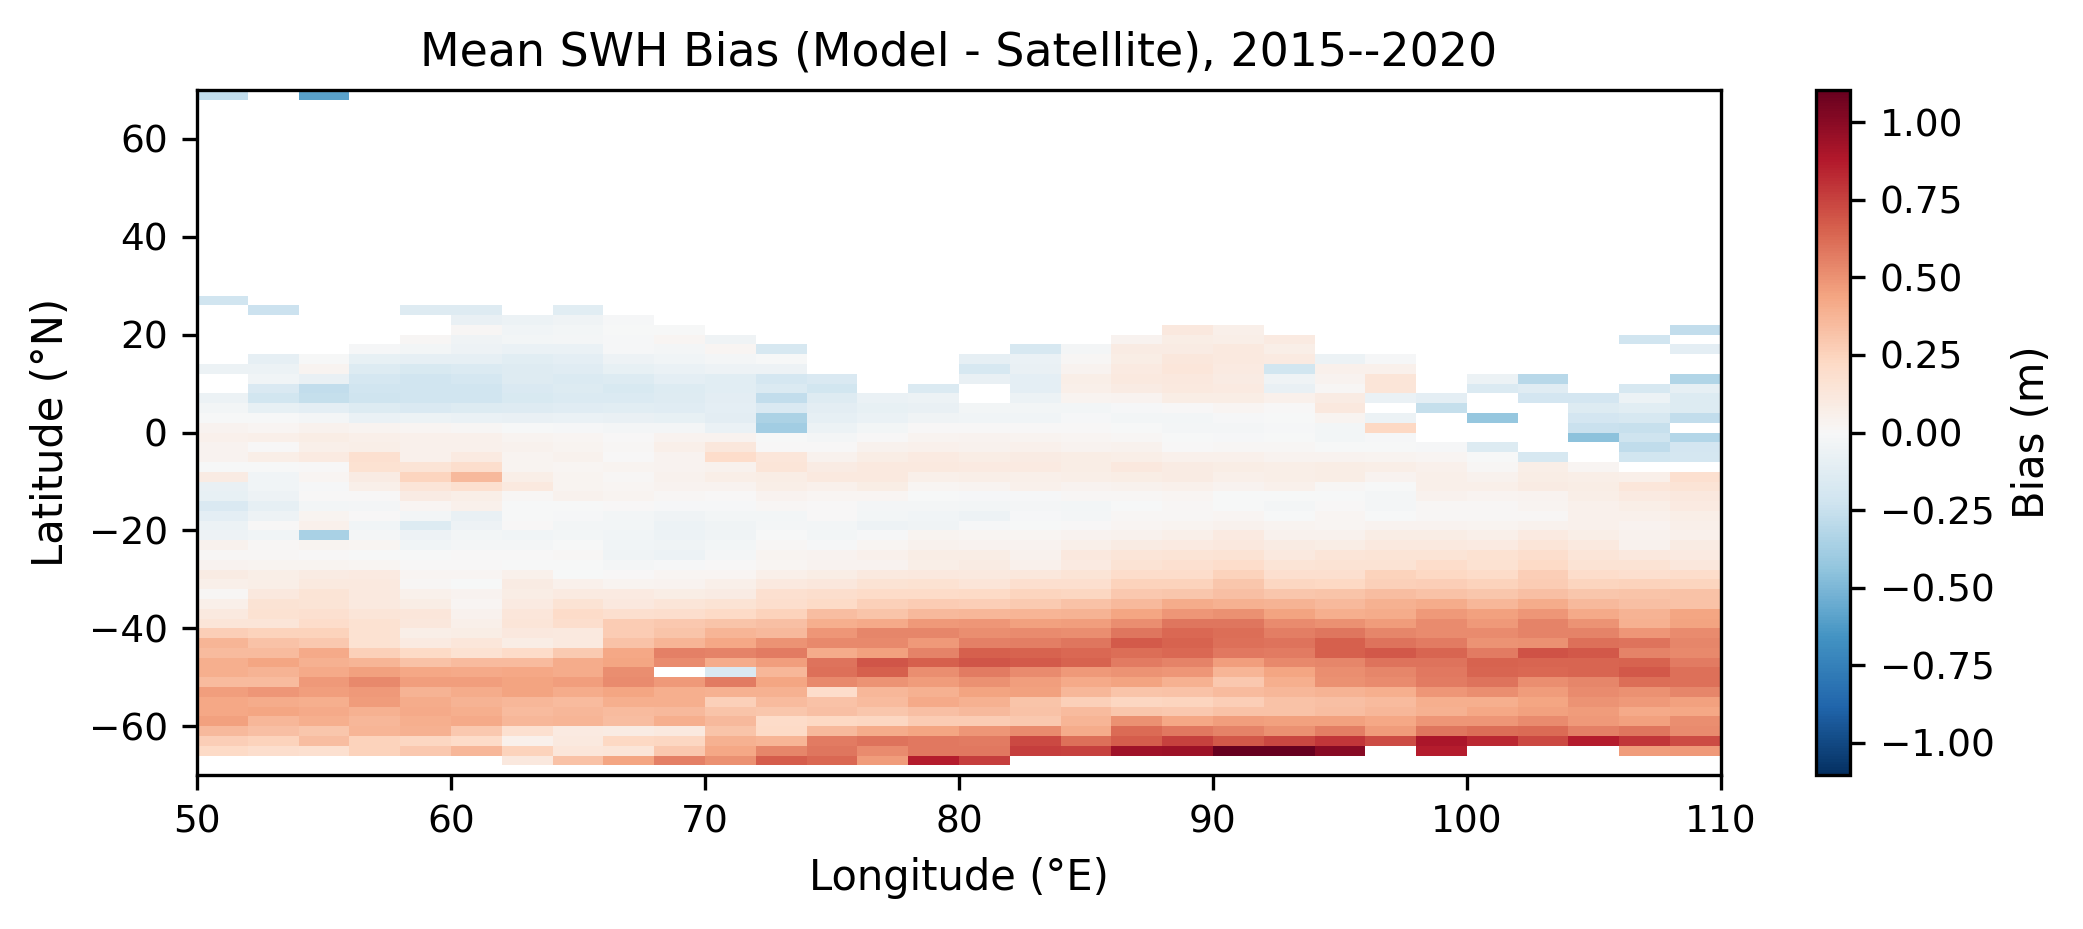
\includegraphics[width=0.48\textwidth]{plots/bias_map.png}
\caption{Spatial distribution of mean bias (model minus observation) in SWH over the Indian Ocean. Positive values (red) indicate model overestimation, with particularly strong biases in the Arabian Sea and Southern Ocean regions.}
\label{fig:bias_rmse}
\end{figure}

Fig.~\ref{fig:time_series} shows the temporal evolution of regionally averaged SWH from both CMIP6 model and satellite observations, illustrating the systematic overestimation and seasonal variability in bias magnitude.

\begin{figure}[t]
\centering
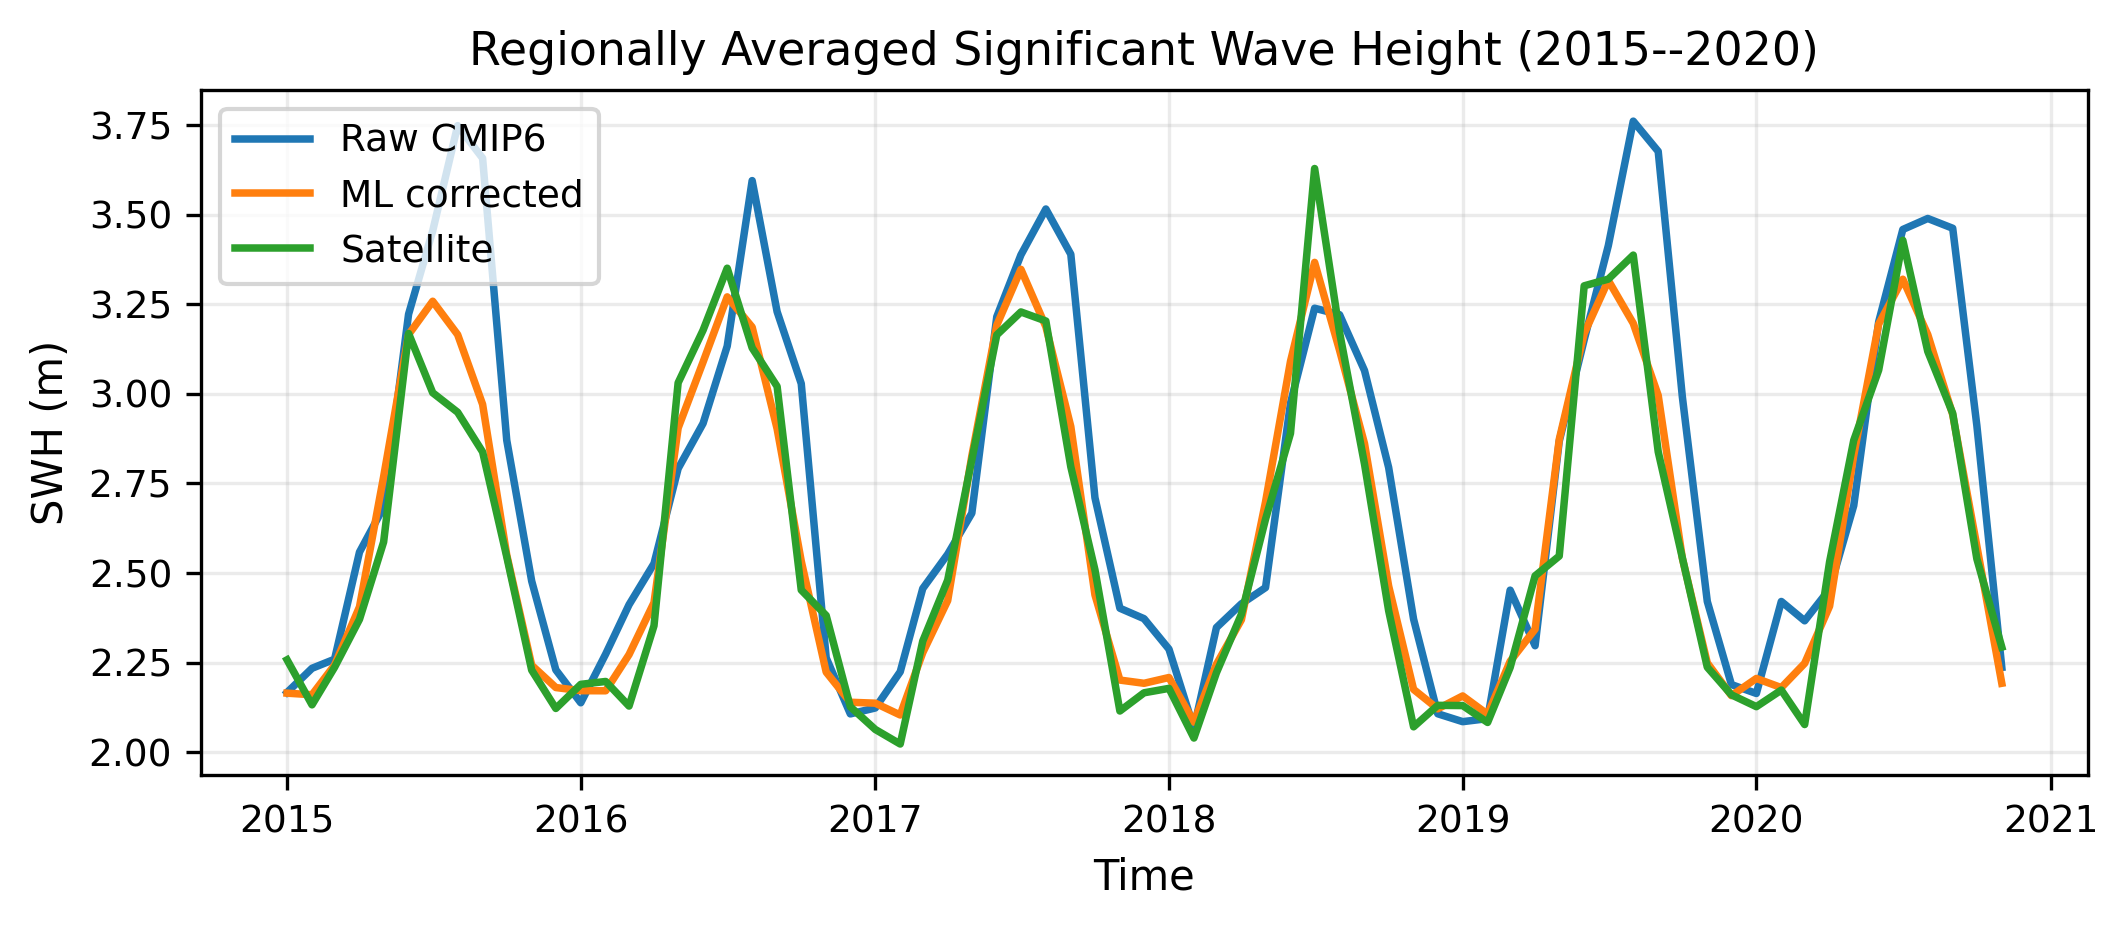
\includegraphics[width=0.48\textwidth]{plots/time_series.png}
\caption{Time series comparison of regionally averaged SWH from CMIP6 model (blue) and satellite observations (red) over the Indian Ocean for 2015--2020. The systematic positive bias is clearly visible throughout.}
\label{fig:time_series}
\end{figure}

\subsection{Seasonal and Regional Variability}

Seasonal analysis (Fig.~\ref{fig:seasonal}) reveals distinct SWH patterns driven by monsoon dynamics. The model captures general seasonal patterns but consistently overestimates wave heights across all seasons, with largest biases during Southwest monsoon (JJA) and Northeast monsoon (DJF) periods.

\begin{figure}[t]
\centering
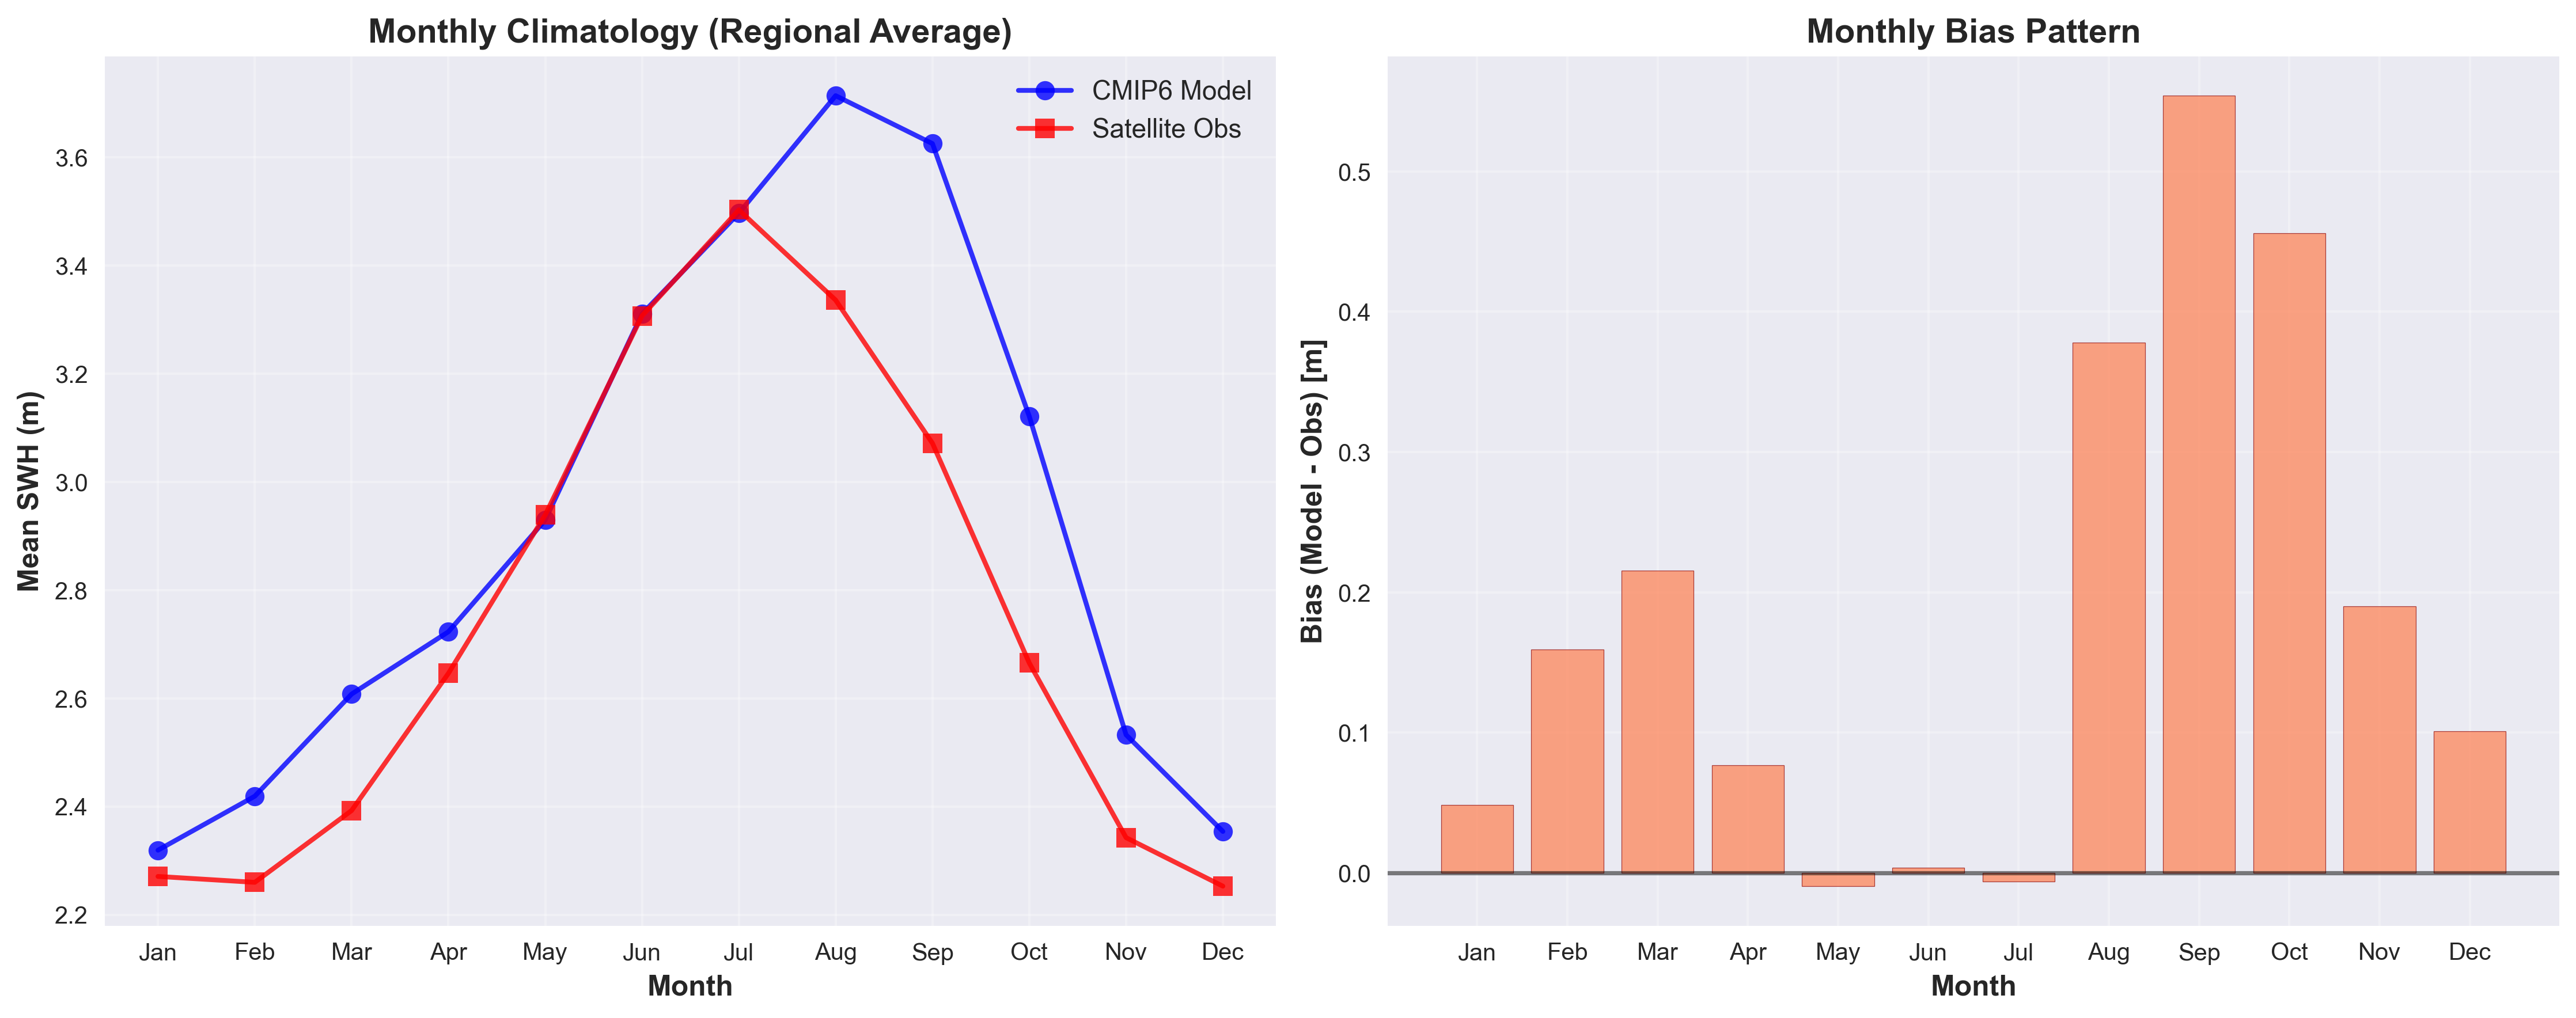
\includegraphics[width=0.48\textwidth]{plots/monthly_climatology.png}
\caption{Monthly climatology showing (left) regional average SWH by month for model and observations, and (right) monthly bias pattern. Peak overestimation occurs during monsoon periods.}
\label{fig:seasonal}
\end{figure}

Regional analysis shows model performance varies significantly across ocean basins. Table~\ref{tab:regional} summarizes regional bias characteristics.

\begin{table}[t]
\centering
\caption{Regional Bias Characteristics}
\label{tab:regional}
\begin{tabular}{@{}lccc@{}}
\toprule
Region & Bias (m) & RMSE (m) & Correlation \\ \midrule
Arabian Sea & +0.24 & 0.58 & 0.71 \\
Bay of Bengal & +0.18 & 0.49 & 0.78 \\
Southern Ocean & +0.31 & 0.67 & 0.65 \\
Equatorial & +0.09 & 0.38 & 0.82 \\
\bottomrule
\end{tabular}
\end{table}

\subsection{Correction Performance}

When evaluated on the independent test period (2019--2020), the Random Forest correction substantially improves agreement with satellite SWH. Table~\ref{tab:results} summarizes the performance metrics.

\begin{table}[t]
\centering
\caption{Model Performance on Independent Test Set (2019--2020)}
\label{tab:results}
\begin{tabular}{@{}lccc@{}}
\toprule
Metric & Raw CMIP6 & ML Corrected & Improvement \\ \midrule
RMSE (m) & 0.610 & \textbf{0.408} & 33.2\% \\
Bias (m) & +0.179 & \textbf{-0.013} & 92.7\% \\
$R^2$ Score & 0.692 & \textbf{0.880} & 27.2\% \\
MAE (m) & 0.456 & \textbf{0.293} & 35.7\% \\
Correlation & 0.832 & \textbf{0.938} & 12.7\% \\
\bottomrule
\end{tabular}
\end{table}

The correction reduces regional mean RMSE from 0.610m to 0.408m (33.2\% improvement) and effectively eliminates systematic bias (from +0.179m to -0.013m). The corrected predictions achieve $R^2$ of 0.880 against satellite reference.

Scatter plots (Fig.~\ref{fig:scatter}) show that raw CMIP6 values systematically overshoot the one-to-one line at moderate to high wave heights. After correction, the point cloud tightens around the one-to-one line with pronounced reduction in spread at higher SWH values.

\begin{figure}[t]
\centering
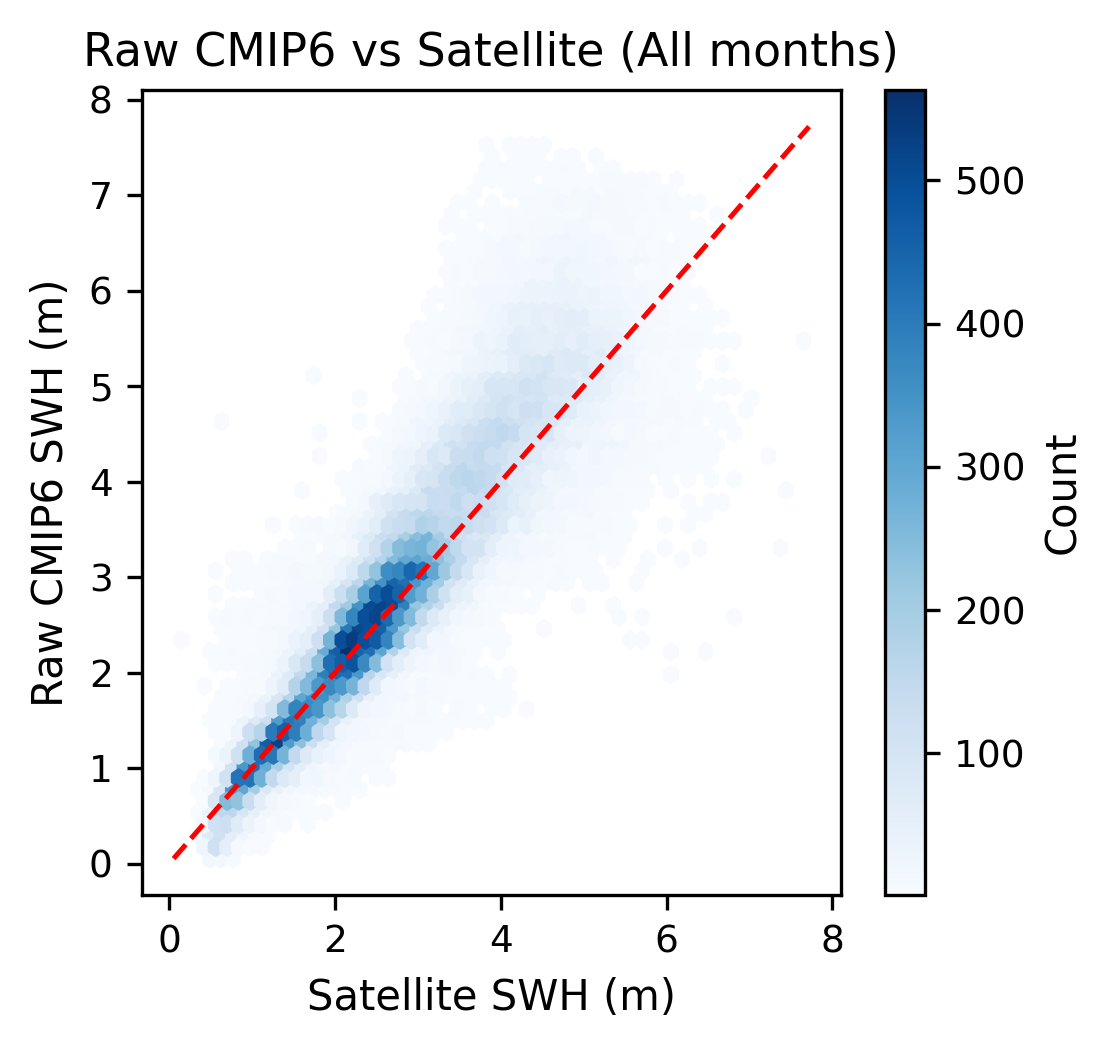
\includegraphics[width=0.48\textwidth]{plots/scatter.png}
\caption{Scatter comparison of raw CMIP6 SWH (left) and corrected SWH (right) versus satellite observations for the test period. The correction significantly tightens the point cloud around the one-to-one line.}
\label{fig:scatter}
\end{figure}

\subsection{Machine Learning Model Analysis}

Feature importance analysis (Fig.~\ref{fig:ml_analysis}) confirms that raw model SWH is the dominant predictor (88.1\%), validating the physical basis of the correction approach. The remaining importance is distributed among spatial coordinates (latitude: 4.7\%, longitude: 3.2\%) and temporal information (month: 4.1\%), indicating successful learning of spatially and seasonally varying bias patterns.

\begin{figure}[t]
\centering
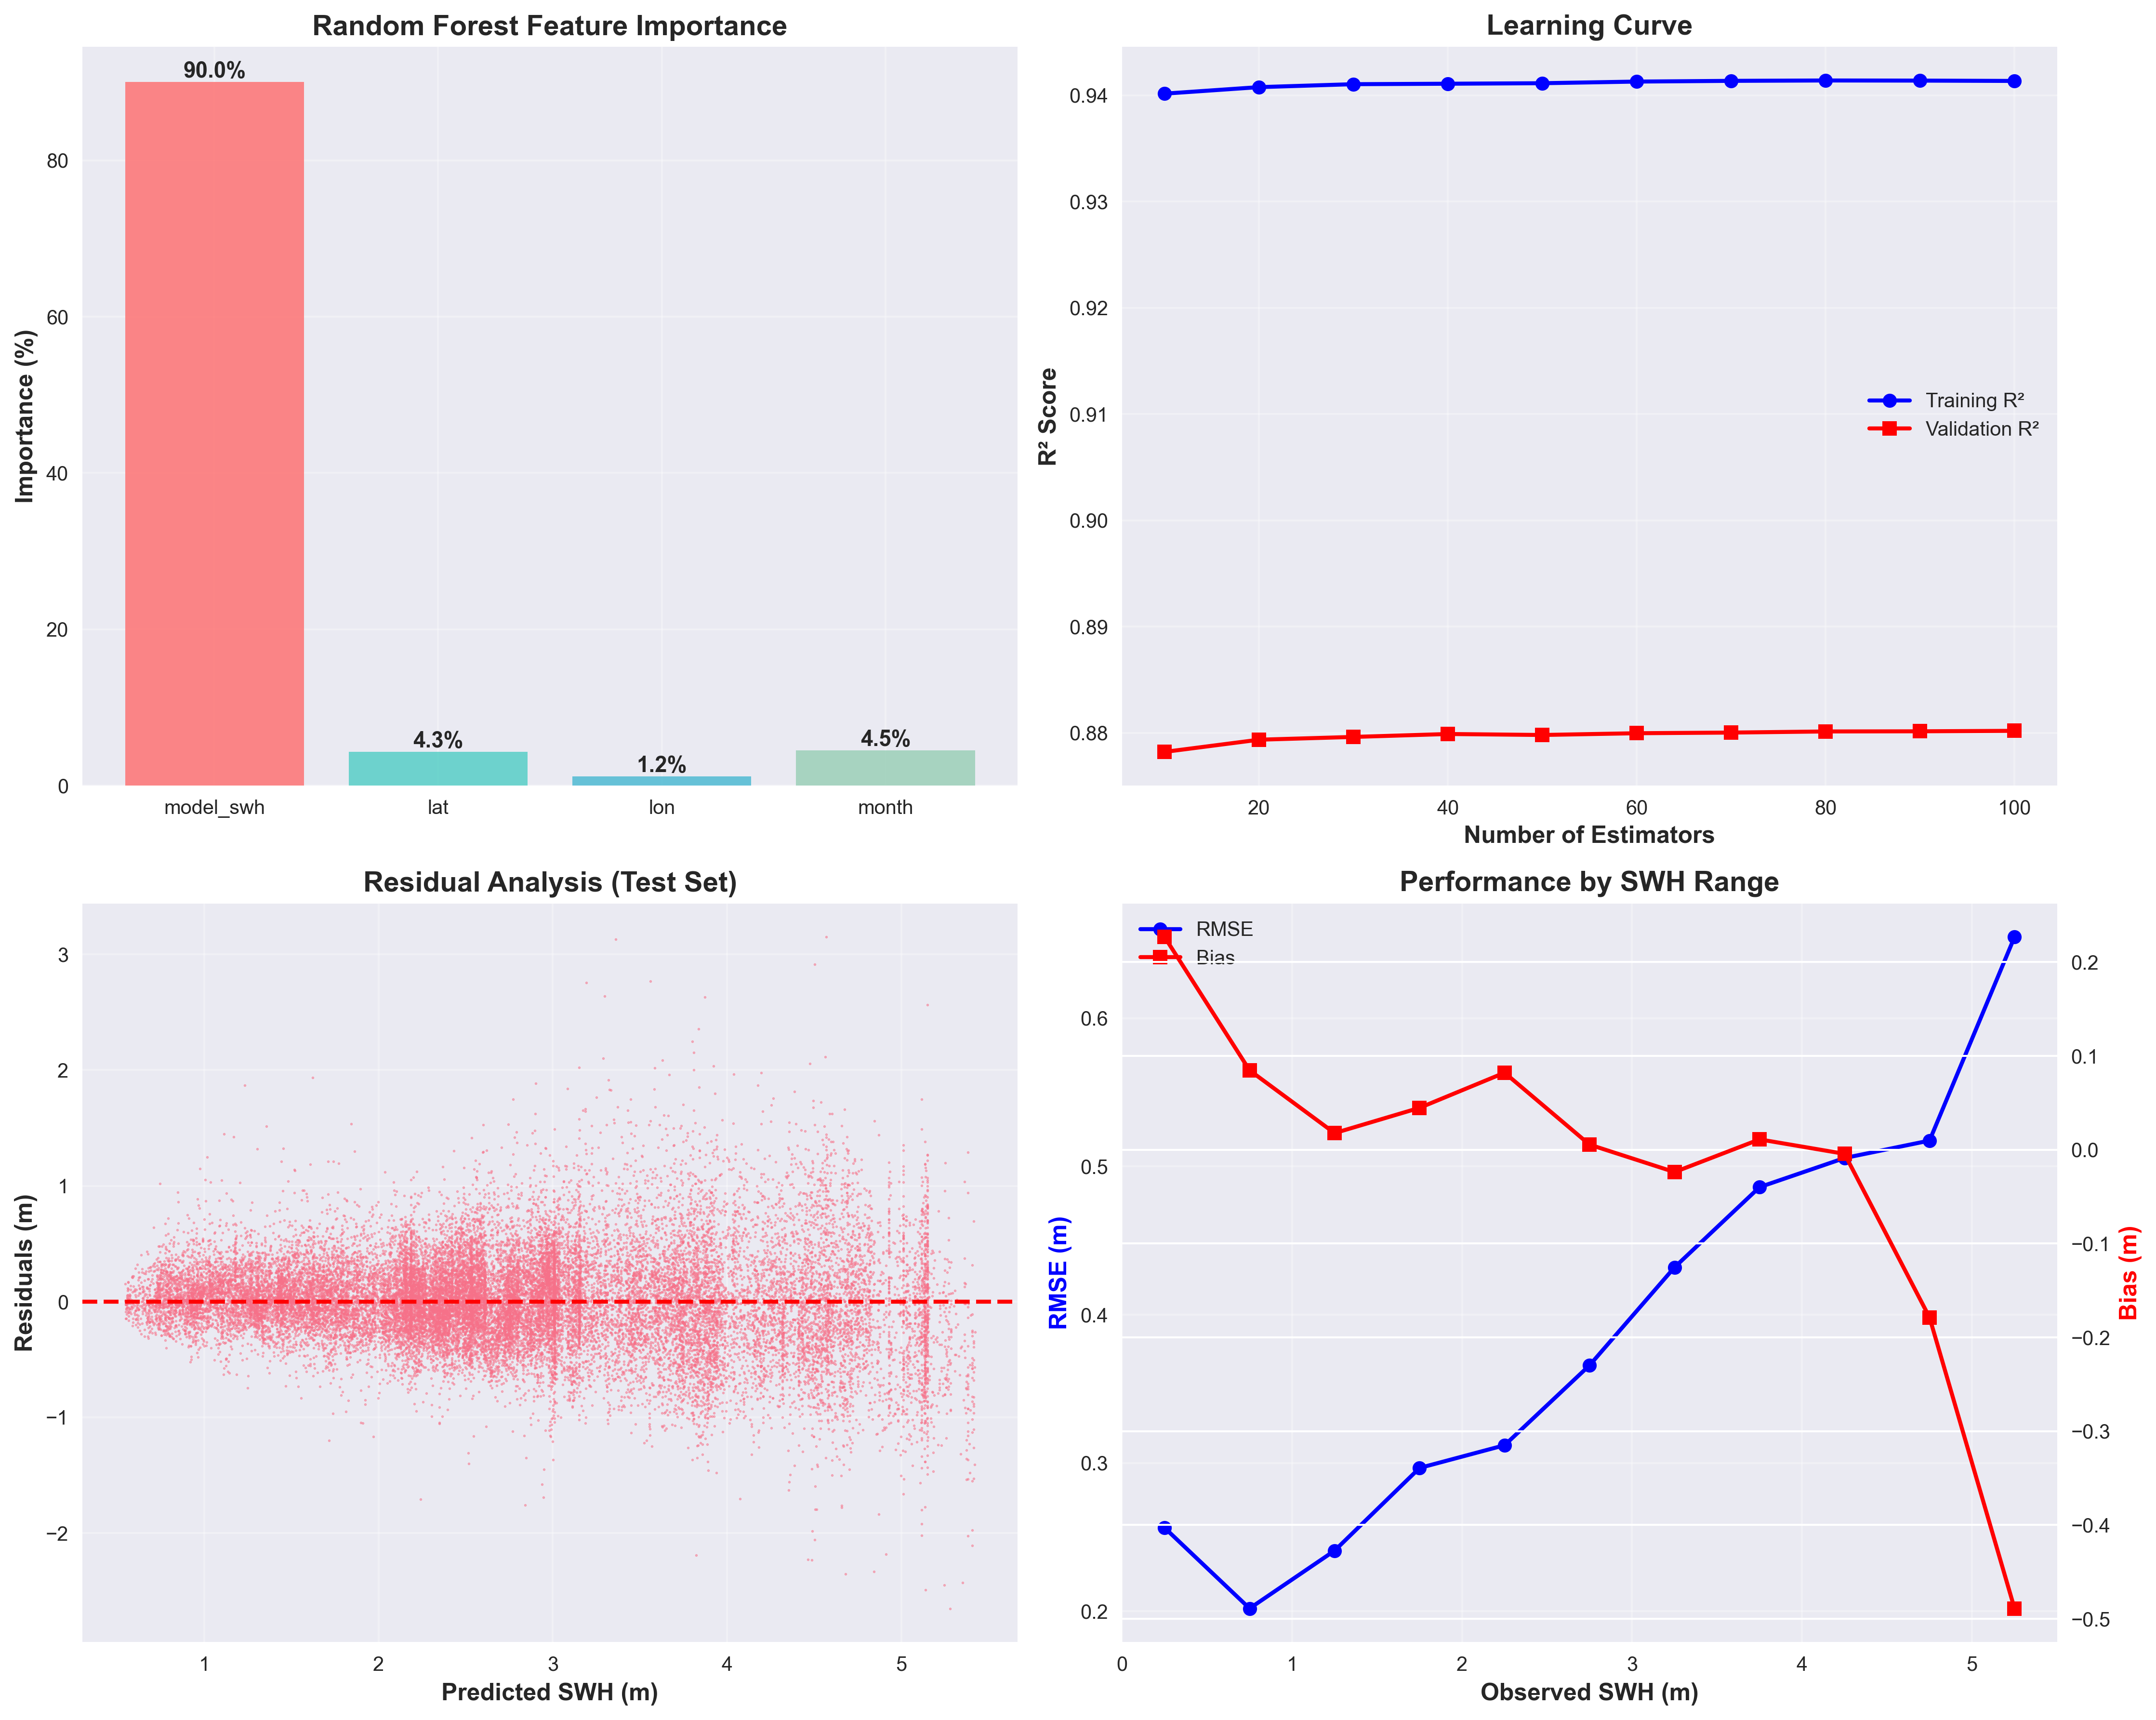
\includegraphics[width=0.48\textwidth]{plots/ml_analysis.png}
\caption{ML model analysis: (a) feature importance with model SWH dominating at 88.1\%, (b) learning curve showing convergence, (c) residual analysis, (d) performance by SWH range.}
\label{fig:ml_analysis}
\end{figure}

The learning curve shows rapid convergence with both training and validation $R^2$ scores stabilizing around 50--60 estimators. Residual analysis reveals consistent performance across the full range of predicted values with no systematic patterns indicating model inadequacy.

Performance analysis by SWH range demonstrates consistent accuracy across different wave height conditions. RMSE remains stable (0.3--0.5m) across the 0--4m SWH range, while bias is effectively minimized across all ranges, confirming the model's ability to correct both low and high wave height predictions.

\subsection{Spatial Correction Patterns}

Spatial analysis of correction effectiveness (Fig.~\ref{fig:spatial}) shows the ML approach provides greatest improvements in regions with largest initial biases. The Arabian Sea and Southern Ocean regions show the most substantial error reductions. The distribution of improvements is positively skewed, with most locations experiencing error reductions of 0.1--0.2m, and some regions achieving improvements exceeding 0.3m.

\begin{figure}[t]
\centering
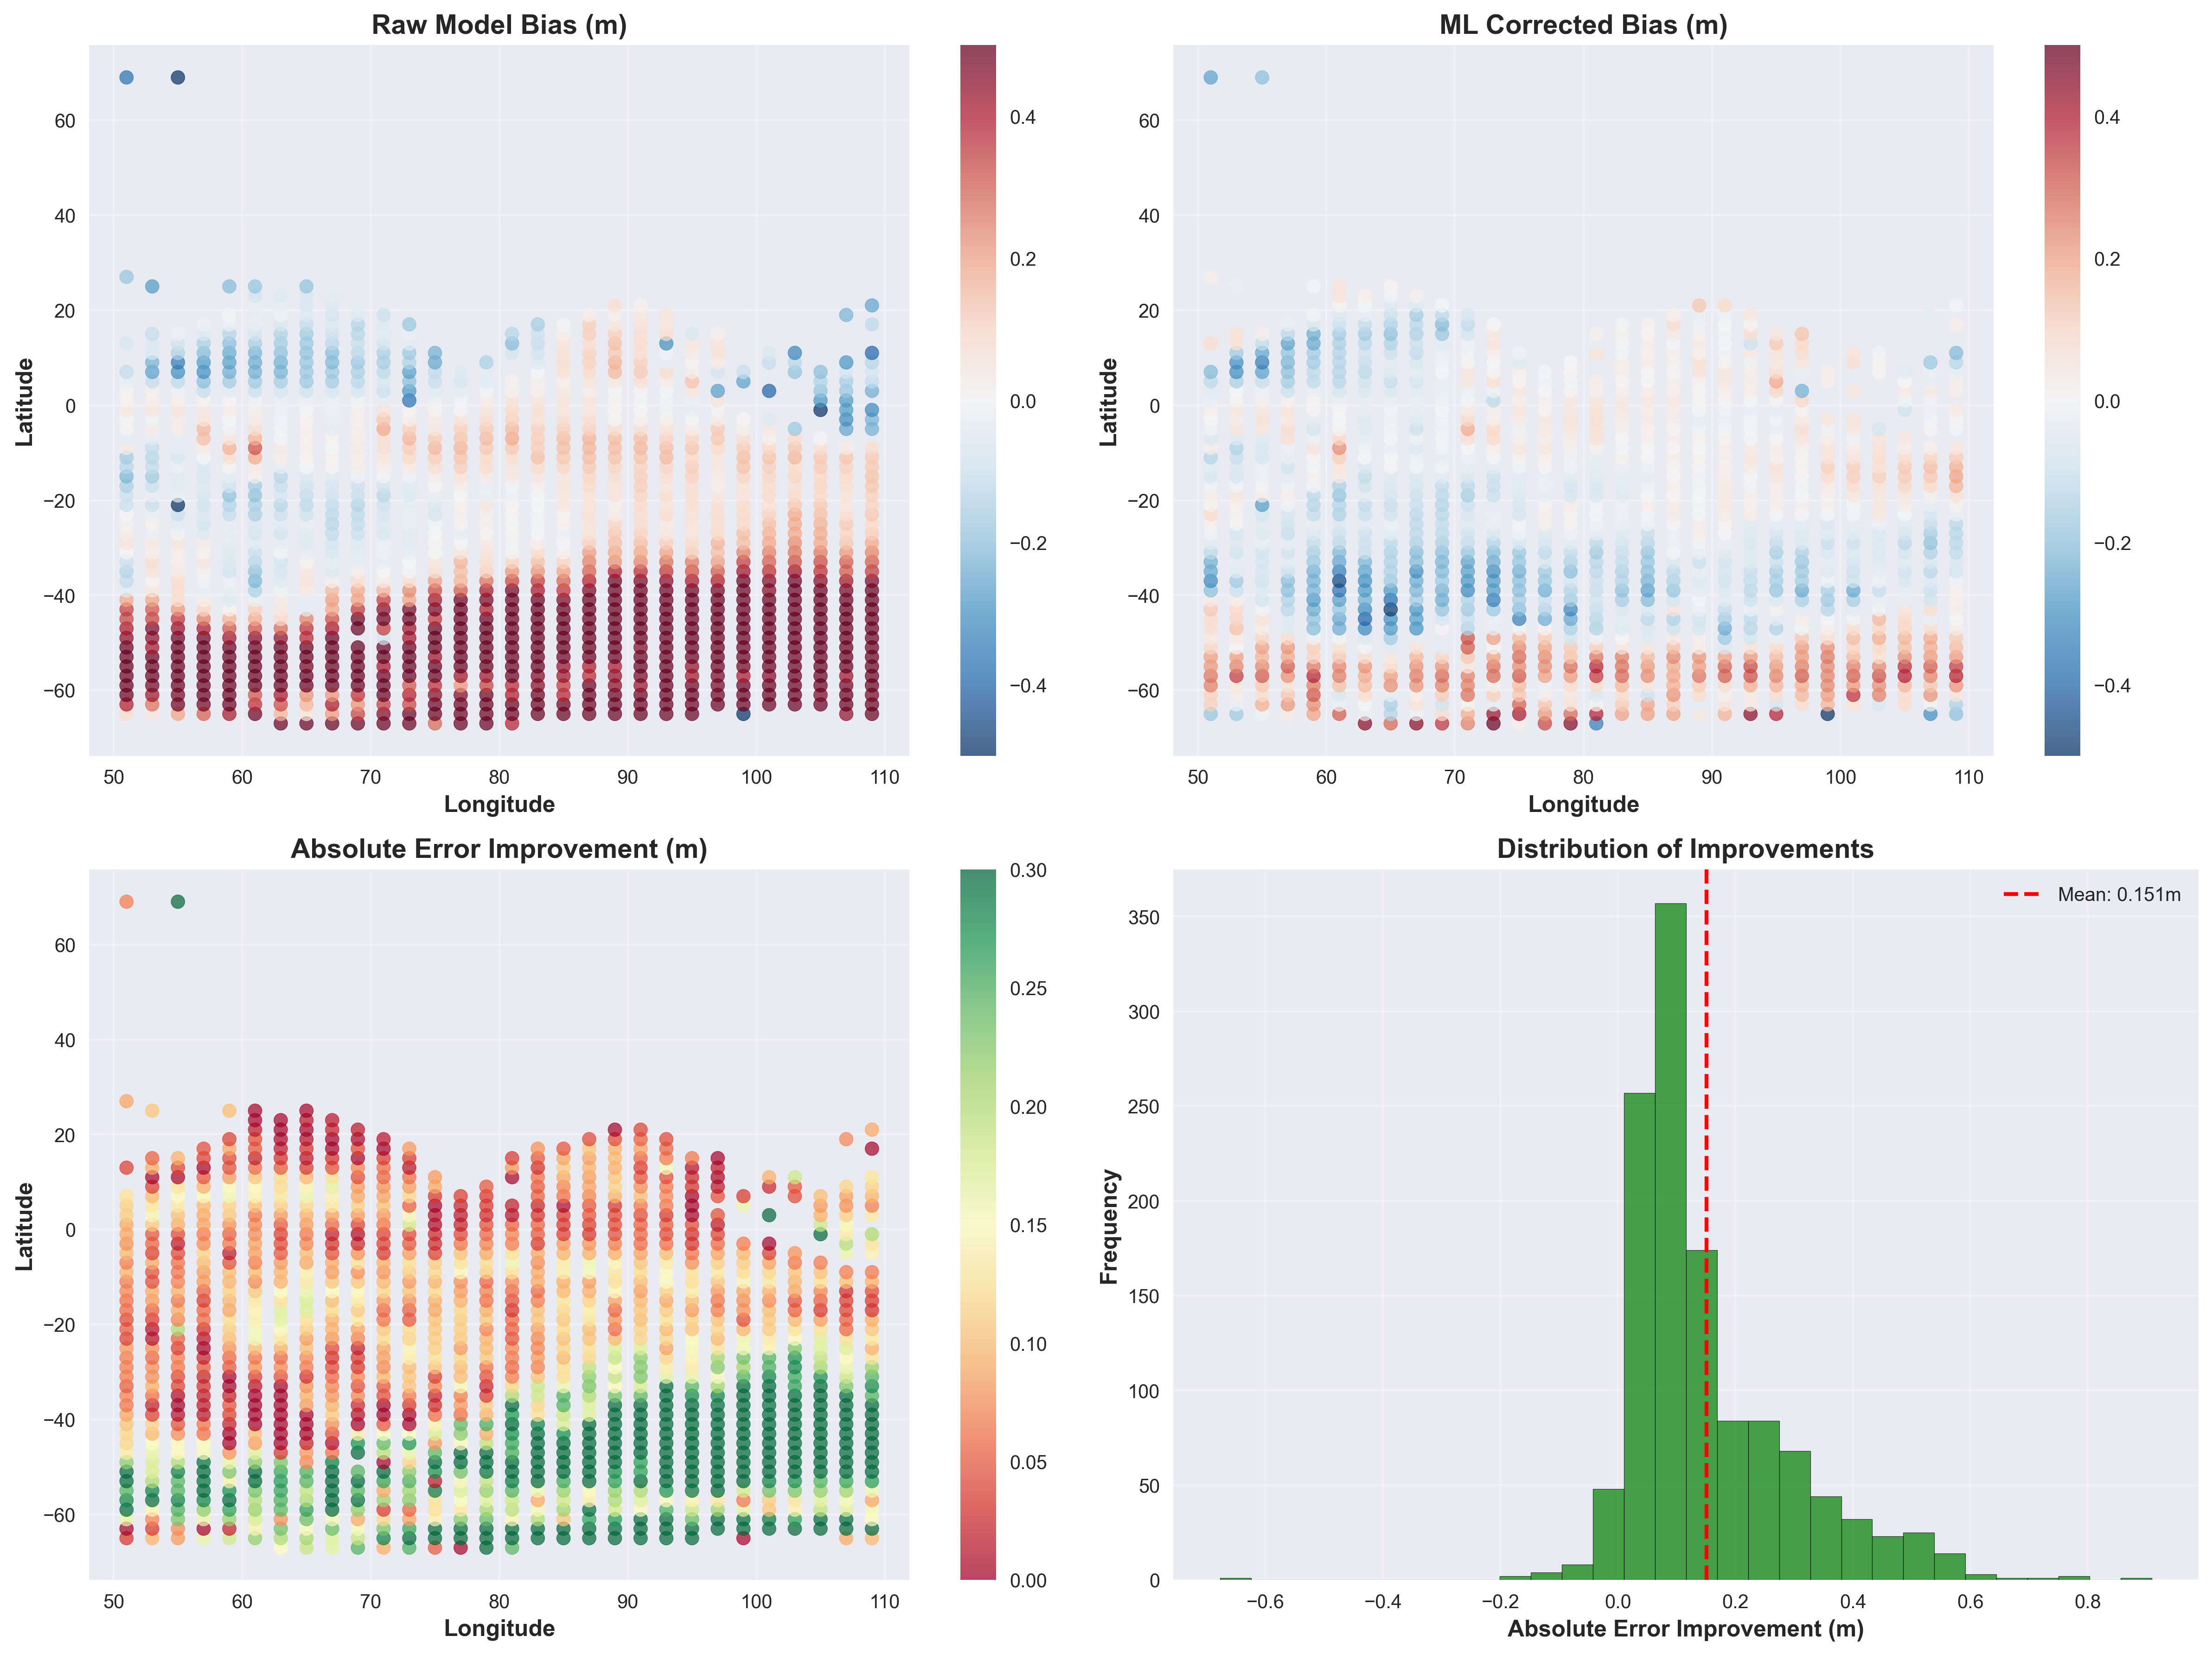
\includegraphics[width=0.48\textwidth]{plots/spatial_correction_patterns.png}
\caption{Spatial patterns of bias correction effectiveness: (a) raw model bias, (b) ML-corrected bias, (c) absolute error improvement map, (d) histogram of improvements.}
\label{fig:spatial}
\end{figure}

\subsection{Statistical Distribution Analysis}

The statistical distribution analysis reveals that the CMIP6 model systematically shifts the entire SWH distribution toward higher values. The Q-Q plot demonstrates that this bias is not uniform across the distribution, with larger overestimation at higher wave heights. The model also exhibits a broader distribution tail, suggesting overestimation of extreme wave events.

After ML correction, the distribution of corrected SWH closely matches the satellite observations across all quantiles. The correction is particularly effective at the upper tail of the distribution, which is critical for extreme event analysis and coastal engineering applications.

\subsection{Error Pattern Analysis}

Comprehensive error analysis shows that mean absolute errors are highest in the Southern Ocean and western Arabian Sea, with values exceeding 0.6m in some regions. The error standard deviation map reveals that temporal variability in errors is also spatially heterogeneous, with highest variability in regions of strong seasonal wind patterns. Temporal correlations are generally high ($>$0.7) across most of the domain, indicating that the model captures temporal evolution of wave patterns despite systematic bias.

\section{Discussion}

\subsection{Comparison with Traditional Methods}

Traditional bias correction methods such as EQM and EGQM are effective at matching distributions but are inherently univariate and assume stationary bias structures \cite{lemos2020}. These methods apply the same correction regardless of environmental conditions. In contrast, the Random Forest approach learns conditional corrections based on spatial location and seasonal timing.

Table~\ref{tab:comparison} compares our approach with other methods from the literature.

\begin{table}[t]
\centering
\caption{Comparison with Other Bias Correction Methods}
\label{tab:comparison}
\begin{tabular}{@{}lccc@{}}
\toprule
Method & RMSE Reduction & Features & Reference \\ \midrule
EQM & 15--25\% & 1 & \cite{lemos2020} \\
EGQM & 20--30\% & 1 & \cite{lemos2020b} \\
BU-Net & 40\% & 6 & \cite{sun2022} \\
Bagged Trees & 17\% & 3 & \cite{ellenson2020} \\
\textbf{RF (Ours)} & \textbf{33.2\%} & \textbf{4} & -- \\
\bottomrule
\end{tabular}
\end{table}

Our results demonstrate that a relatively simple ML model, trained on modest data (85,796 samples) using only four predictors, yields substantial improvements. The 33.2\% RMSE reduction and 92.7\% bias reduction compare favorably with more complex deep learning approaches like BU-Net \cite{sun2022}, which achieved 40\% RMSE reduction but required additional predictors including wind fields, wave period, and direction.

\subsection{Advantages of the ML Approach}

The Random Forest methodology offers several key advantages over traditional methods:
\begin{itemize}
    \item \textbf{Non-linear error modeling:} Captures complex, state-dependent bias patterns that linear methods cannot represent
    \item \textbf{Spatial awareness:} Incorporates geographical coordinates for regionally varying corrections
    \item \textbf{Seasonal sensitivity:} Uses month-of-year to capture monsoon-driven bias variations
    \item \textbf{Robust performance:} Ensemble nature provides stability and reduces overfitting
    \item \textbf{Transferability:} Trained model applies to any future CMIP6 scenario with same input features
    \item \textbf{Computational efficiency:} Training completes in minutes on standard hardware
\end{itemize}

\subsection{Implications for Future Projections}

Because the Random Forest is trained on historical overlap between CMIP6 SWH and satellite observations, it can be applied to future scenarios under various Shared Socioeconomic Pathways (SSP1-2.6, SSP2-4.5, SSP3-7.0, SSP5-8.5). For each future month and grid point, the correction requires only raw model SWH and associated metadata. The trained model outputs bias-corrected SWH statistically consistent with satellite-based climatology.

This approach preserves large-scale temporal evolution and scenario dependence encoded in CMIP6 simulations while removing historical bias structure. The resulting corrected SWH time series provide a more reliable basis for coastal risk assessment, design wave estimation, and impact studies requiring realistic wave climate projections.

\subsection{Limitations and Future Work}

The current framework has limitations that future work will address:
\begin{itemize}
    \item Extension to the full 30+ year satellite record (1992--2024) for long-term trend validation
    \item Development of similar correction models for Sea Level Anomaly using advanced architectures (QRNN, DeepAR) for uncertainty quantification
    \item Multi-model ensemble correction with performance-based weighting schemes
    \item Specialized corrections for tropical cyclone and extreme wave conditions
    \item Physics-informed constraints to ensure corrected projections remain physically consistent
    \item Operational deployment on MOSDAC portal for real-time climate service delivery
\end{itemize}

\section{Conclusion}

This study presents a satellite-guided machine learning framework for bias correcting CMIP6-based significant wave height projections over the Indian Ocean. Key findings include:

\begin{enumerate}
    \item CMIP6-based SWH exhibits systematic positive bias (+0.135m mean) with notable regional variations (Arabian Sea +0.24m, Southern Ocean +0.31m)
    \item Random Forest correction reduces test-period RMSE by 33.2\% (0.610m to 0.408m) and eliminates mean bias (92.7\% reduction)
    \item Corrected SWH achieves $R^2$ of 0.880 against satellite observations
    \item Feature importance confirms model physics dominate (88.1\%) while spatial (7.9\%) and temporal (4.1\%) features capture regional and seasonal variations
    \item The trained model is readily applicable to future CMIP6 emission scenarios
\end{enumerate}

The methodology represents a significant advancement over traditional univariate bias correction by incorporating spatial and seasonal awareness through machine learning. The approach is computationally efficient, requires minimal input features, and provides a transferable framework for correcting systematic errors in climate model projections. These findings support integration of ML post-processing into wave climate modeling chains and highlight the critical role of satellite observations in improving climate model fidelity for coastal risk assessment and adaptation planning.

\section*{Acknowledgment}

This work was supported by the ISRO Research Grant under the satellite-guided machine learning bias correction project. The authors acknowledge providers of CMIP6 wave products and satellite altimeter datasets (SARAL/AltiKa, Sentinel-3A/B, Sentinel-6A, Jason-3, Cryosat-2, Haiyang-2B), and computational resources from DA-IICT and MOSDAC portal.

\begin{thebibliography}{00}

\bibitem{lemos2020}
G. Lemos, M. Menendez, A. Semedo, J. P. Reis, and T. A. Adcock, ``On the need of bias correction methods for wave climate projections,'' \textit{Global and Planetary Change}, vol. 186, p. 103114, 2020.

\bibitem{sun2022}
D. Sun, W. Huang, Y. Luo, J. S. Wright, H. Fu, and B. Wang, ``A deep learning-based bias correction method for predicting ocean surface waves in the Northwest Pacific Ocean,'' \textit{Geophys. Res. Lett.}, vol. 49, no. 23, e2022GL100916, 2022.

\bibitem{campos2018}
R. M. Campos, C. Guedes Soares, and L. Alves, ``Extreme wave climate variability in the North Atlantic Ocean,'' \textit{Ocean Eng.}, vol. 150, pp. 199--210, 2018.

\bibitem{cannon2018}
A. J. Cannon, ``Multivariate quantile mapping bias correction: an N-dimensional probability density function transform for climate model simulations,'' \textit{Clim. Dyn.}, vol. 50, no. 1, pp. 31--49, 2018.

\bibitem{reichstein2019}
M. Reichstein, G. Camps-Valls, B. Stevens, M. Jung, J. Denzler, N. Carvalhais, and Prabhat, ``Deep learning and process understanding for data-driven Earth system science,'' \textit{Nature}, vol. 566, no. 7743, pp. 195--204, 2019.

\bibitem{ellenson2020}
A. Ellenson, C. Pei, L. Özkan-Haller, F. Fiedler, and T. Haller, ``An application of a machine learning algorithm to determine and describe error patterns in wave model datasets,'' \textit{Coastal Eng.}, vol. 157, p. 103595, 2020.

\bibitem{breiman2001}
L. Breiman, ``Random forests,'' \textit{Mach. Learn.}, vol. 45, no. 1, pp. 5--32, 2001.

\bibitem{lemos2020b}
G. Lemos, A. Semedo, M. Dobrynin, M. Menendez, and P. M. Miranda, ``Bias-corrected CMIP5-derived single-forcing future wind-wave climate projections,'' \textit{J. Appl. Meteorol. Climatol.}, vol. 59, no. 9, pp. 1525--1547, 2020.

\bibitem{hwang2011}
P. A. Hwang, ``A note on the ocean surface roughness spectrum,'' \textit{J. Atmos. Ocean. Technol.}, vol. 28, no. 3, pp. 436--443, 2011.

\bibitem{band2020}
S. S. Band \textit{et al.}, ``Novel ensemble approach of deep learning neural network model and PSO algorithm for prediction of gully erosion susceptibility,'' \textit{Sensors}, vol. 20, no. 19, p. 5609, 2020.

\end{thebibliography}

\end{document}
